\documentclass[12pt,a4paper]{report}
\usepackage[utf8]{inputenc}
\usepackage[russian]{babel}
\usepackage[OT1]{fontenc}
\usepackage{amsmath}
\usepackage{amsfonts}
\usepackage{amssymb}
\usepackage{graphicx}
\usepackage{cmap}					% поиск в PDF
\usepackage{mathtext} 				% русские буквы в формулах
%\usepackage{tikz-uml}               % uml диаграммы
\usepackage [ section ]{ placeins}
% TODOs
\usepackage[%
  colorinlistoftodos,
  shadow
]{todonotes}

% Генератор текста
\usepackage{blindtext}

%------------------------------------------------------------------------------

% Подсветка синтаксиса
\usepackage{color}
\usepackage{xcolor}
\usepackage{listings}
 
 % Цвета для кода
\definecolor{string}{HTML}{B40000} % цвет строк в коде
\definecolor{comment}{HTML}{008000} % цвет комментариев в коде
\definecolor{keyword}{HTML}{1A00FF} % цвет ключевых слов в коде
\definecolor{morecomment}{HTML}{8000FF} % цвет include и других элементов в коде
\definecolor{captiontext}{HTML}{FFFFFF} % цвет текста заголовка в коде
\definecolor{captionbk}{HTML}{999999} % цвет фона заголовка в коде
\definecolor{bk}{HTML}{FFFFFF} % цвет фона в коде
\definecolor{frame}{HTML}{999999} % цвет рамки в коде
\definecolor{brackets}{HTML}{B40000} % цвет скобок в коде
 
 % Настройки отображения кода
\lstset{
language=C, % Язык кода по умолчанию
morekeywords={*,...}, % если хотите добавить ключевые слова, то добавляйте
 % Цвета
keywordstyle=\color{keyword}\ttfamily\bfseries,
stringstyle=\color{string}\ttfamily,
commentstyle=\color{comment}\ttfamily\itshape,
morecomment=[l][\color{morecomment}]{\#}, 
 % Настройки отображения     
breaklines=true, % Перенос длинных строк
basicstyle=\ttfamily\footnotesize, % Шрифт для отображения кода
backgroundcolor=\color{bk}, % Цвет фона кода
%frame=lrb,xleftmargin=\fboxsep,xrightmargin=-\fboxsep, % Рамка, подогнанная к заголовку
frame=tblr
rulecolor=\color{frame}, % Цвет рамки
tabsize=3, % Размер табуляции в пробелах
 % Настройка отображения номеров строк. Если не нужно, то удалите весь блок
numbers=left, % Слева отображаются номера строк
stepnumber=1, % Каждую строку нумеровать
numbersep=5pt, % Отступ от кода 
numberstyle=\small\color{black}, % Стиль написания номеров строк
 % Для отображения русского языка
extendedchars=true,
literate={Ö}{{\"O}}1
  {Ä}{{\"A}}1
  {Ü}{{\"U}}1
  {ß}{{\ss}}1
  {ü}{{\"u}}1
  {ä}{{\"a}}1
  {ö}{{\"o}}1
  {~}{{\textasciitilde}}1
  {а}{{\selectfont\char224}}1
  {б}{{\selectfont\char225}}1
  {в}{{\selectfont\char226}}1
  {г}{{\selectfont\char227}}1
  {д}{{\selectfont\char228}}1
  {е}{{\selectfont\char229}}1
  {ё}{{\"e}}1
  {ж}{{\selectfont\char230}}1
  {з}{{\selectfont\char231}}1
  {и}{{\selectfont\char232}}1
  {й}{{\selectfont\char233}}1
  {к}{{\selectfont\char234}}1
  {л}{{\selectfont\char235}}1
  {м}{{\selectfont\char236}}1
  {н}{{\selectfont\char237}}1
  {о}{{\selectfont\char238}}1
  {п}{{\selectfont\char239}}1
  {р}{{\selectfont\char240}}1
  {с}{{\selectfont\char241}}1
  {т}{{\selectfont\char242}}1
  {у}{{\selectfont\char243}}1
  {ф}{{\selectfont\char244}}1
  {х}{{\selectfont\char245}}1
  {ц}{{\selectfont\char246}}1
  {ч}{{\selectfont\char247}}1
  {ш}{{\selectfont\char248}}1
  {щ}{{\selectfont\char249}}1
  {ъ}{{\selectfont\char250}}1
  {ы}{{\selectfont\char251}}1
  {ь}{{\selectfont\char252}}1
  {э}{{\selectfont\char253}}1
  {ю}{{\selectfont\char254}}1
  {я}{{\selectfont\char255}}1
  {А}{{\selectfont\char192}}1
  {Б}{{\selectfont\char193}}1
  {В}{{\selectfont\char194}}1
  {Г}{{\selectfont\char195}}1
  {Д}{{\selectfont\char196}}1
  {Е}{{\selectfont\char197}}1
  {Ё}{{\"E}}1
  {Ж}{{\selectfont\char198}}1
  {З}{{\selectfont\char199}}1
  {И}{{\selectfont\char200}}1
  {Й}{{\selectfont\char201}}1
  {К}{{\selectfont\char202}}1
  {Л}{{\selectfont\char203}}1
  {М}{{\selectfont\char204}}1
  {Н}{{\selectfont\char205}}1
  {О}{{\selectfont\char206}}1
  {П}{{\selectfont\char207}}1
  {Р}{{\selectfont\char208}}1
  {С}{{\selectfont\char209}}1
  {Т}{{\selectfont\char210}}1
  {У}{{\selectfont\char211}}1
  {Ф}{{\selectfont\char212}}1
  {Х}{{\selectfont\char213}}1
  {Ц}{{\selectfont\char214}}1
  {Ч}{{\selectfont\char215}}1
  {Ш}{{\selectfont\char216}}1
  {Щ}{{\selectfont\char217}}1
  {Ъ}{{\selectfont\char218}}1
  {Ы}{{\selectfont\char219}}1
  {Ь}{{\selectfont\char220}}1
  {Э}{{\selectfont\char221}}1
  {Ю}{{\selectfont\char222}}1
  {Я}{{\selectfont\char223}}1
  {і}{{\selectfont\char105}}1
  {ї}{{\selectfont\char168}}1
  {є}{{\selectfont\char185}}1
  {ґ}{{\selectfont\char160}}1
  {І}{{\selectfont\char73}}1
  {Ї}{{\selectfont\char136}}1
  {Є}{{\selectfont\char153}}1
  {Ґ}{{\selectfont\char128}}1
  {\{}{{{\color{brackets}\{}}}1 % Цвет скобок {
  {\}}{{{\color{brackets}\}}}}1 % Цвет скобок }
}
 
 % Для настройки заголовка кода
\usepackage{caption}
\DeclareCaptionFont{white}{\color{сaptiontext}}
\DeclareCaptionFormat{listing}{\parbox{\linewidth}{\colorbox{сaptionbk}{\parbox{\linewidth}{#1#2#3}}\vskip-4pt}}
\captionsetup[lstlisting]{format=listing,labelfont=white,textfont=white}
\renewcommand{\lstlistingname}{Код} % Переименование Listings в нужное именование структуры
\DeclareGraphicsExtensions{.pdf,.png,.jpg}



%------------------------------------------------------------------------------

\author{К.~Е.~Назарова}
\title{Сети ЭВМ и телекоммуникации}
\begin{document}
\listoftodos
\maketitle
\chapter{Информационная система}
\section{Функциональные требования}
\subsection{Задание}
Разработать распределённую информационную систему, состоящую из приложения-сервера и приложения-клиента. Информационная система является иерархическим хранилищем статей, каждая из которых состоит из названия, автора и текста статьи. Информационная система должна обеспечивать параллельный доступ к информации нескольким клиентам.
\subsection{Основные возможности}
Серверное приложение должно реализовывать следующие функции:
\begin{enumerate}
\item Прослушивание определенного порта
\item Обработка запросов на подключение по этому порту от клиентов
\item Поддержка одновременной работы нескольких клиентов через механизм нитей

%\item Хранение иерархической структуры статей информационной системы
\item Передача пользователю списка текущих разделов системы, списка статей
\item Переход в конкретный раздел системы по запросу клиента
\item Возврат на предыдущий уровень по запросу клиента
\item Передача пользователю конкретной статьи по названию
\item Передача пользователю всех статей текущего раздела, принадлежащих определенному автору
\item Приём от клиента новой статьи и сохранение в информационной системе
\item Обработка запроса на отключение клиента
\item Принудительное отключение клиента
\end{enumerate}
Клиентское приложение должно реализовывать следующие функции:
\begin{enumerate}
\item Установление соединения с сервером
\item Получение и печать списка подразделов и статей раздела
\item Передача команды на переход в конкретный раздел
\item Передача команды на переход в раздел на уровень выше
\item Получение конкретной статьи из информационной системы
\item Получение статей конкретного автора
\item Посылка новой статьи в систему
\item Разрыв соединения
\item Обработка ситуации отключения клиента сервером 
\end{enumerate}
\subsection{Настроки приложений}
Разработанное клиентское приложение предоставляет пользователю возможность введения настройки IP-адреса или доменного имени, а также номера порта сервера информационной системы.
\section{Нефункциональные требования}
\subsection{Требования к реализаии}
Соединение начинает клиент. При подключении к порту и отправке начального сообщения, сервер передает клиенту список доступных разделов статей (содержимое корневой директории). Информационная система имеет иерархическую структуру, что позволяет киенту переходить в конкретный раздел системы и возвращаться на предыдущий уровень. В ходе соединения клиент имеет возможность читать любые статьи, задавать поиск по автору статьи в конкретном разделе, а также добавлять статьи в раздел. 
%\subsection{Требования к надежности}
%Требования к производительности, надежности, целевым платформам и~т.п.
\section{Накладываемые ограничения}
\begin{enumerate}
\item Ограничения на длину пакета
MSS (Maximum segment size) является параметром протокола TCP и определяет максимальный размер полезного блока данных в байтах для TCP пакета (сегмента). Таким образом этот параметр не учитывает длину заголовков TCP и IP. Для установления корректной TCP сессии с удалённым хостом должно соблюдаться следующее условие:
\begin{equation}
	MSS + заголовок TCP + заголовок IP <= MTU
\end{equation}
Таким образом, максимальный размер MSS = MTU — размер заголовка IPv4 — размер заголовка TCP
В данной реализации длина пакета составляет 1024 байта. Это объясняется там, что значение MSS обеих используемх операционных систем равно 1500 октетов:
\begin{figure}[h]
\center{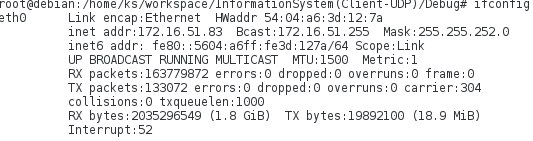
\includegraphics[width=1\linewidth]{mtu_unix}}
\caption{Значение MTU для ОС Unix}
\label{fig:mtu_unix}
\end{figure}
\begin{figure}[h]
\center{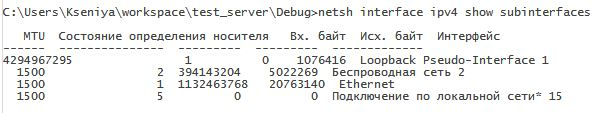
\includegraphics[width=1\linewidth]{mtu_win.JPG}}
\caption{Значение MTU для ОС Windows 8}
\label{fig:mtu_win}
\end{figure}
\item Ограничения на длину статьи
На данном этапе максимальная длина статьи составляет 4096 байт. Такое значение выбрано для удобства реализации UDP-соединения, а также для простоты тестирования и отладки.
\item Ограничения на переход клиентом из родительской директории информационной системы на уровень выше.
\item Количество файлов в разделе. Их максимальное значение равно 100. Такое значение взято для удобного поиска по автору статьи.
\item Разрыв соединения, при котором теряются введенные клиентом запросы и данные, и при очередом подключении он снова оказывается в корневой директории, а статья, которую он создавал, не сохранилась.
\item Сервер и клиент не оповещают друг друга о потере связи.
\item Не до конца реализовано параллельное соединение клиентов в UDP. На данном этапе при подключении кажды следующий клиент должен дождаться завершения работы предыдущего.
\end{enumerate}
\chapter{Реализация для работы по протоколу TCP}
\section{Прикладной протокол}
\label{protocol_tcp}
Соединение начинается с задания ip-адреса и номера порта. Для этого используются ключи -p:\{№порта\} -i:\{ip-адрес\}.
По умолчанию используется порт №5001 и соединение с localhost (127.0.0.1).\\ \\
\hspace*{-5em} 
\begin{tabular}{c|c}
\hline
\multicolumn{2}{c}{\textbf{Пользовательские команды}}\\
\hline 
\small Команда &\small Назначение \\ 
\hline 
\small :start &\small Оповещение сервера о начале работы \\ 

\small open [файл | директория | . | .. ] & \small Позволяет открывать файлы и перемещаться медлу разделами \\ 

\small find [автор] & \small Команда поиска статей по имени автора в текущем разделе\\ 

\small add[Заголовок][Автор][Содержимое][:end] &\small Команда для добавления новой статьи в текущую директорию \\ 
 
\small :end & \small Оповещение о конце ввода новой статьи \\ 

\small :exit &\small Оповещение о разрыве соединения клиентом \\ 
\hline
\end{tabular} 
\\ 
\\Все команды вводятся в текстовом формате. При этом накладываются следующие ограничения на длину параметров команд:\\
\\
\begin{tabular}{|c|c|c|}
\hline 
Команда & Параметр & Формат \\ 
\hline 
open & файл & char [1024] \\ 
 
  & директория & char [1024] \\ 

  & родительская директория & .. \\ 

  & текущая директория & . \\ 
\hline 
find & автор & char [128] \\ 
\hline 
add & заголовок & char [128] \\ 

  & автор & char [128] \\ 
 
  & содержимое & char [4096] \\ 
\hline 
\end{tabular} 

\section{Архитектура приложения}

\hspace*{2em} При начальном подключении протокол имеет возмжность введения настройки ip-адреса или доменного имени и номера порта сервера информационной системы.  
\\ 
\hspace*{2em} Сама информационная система расположена на сервере в каталоге "./Information System/" и состоит из каталогово и txt-файлов. При получении сообщения от клиента к серверу о соединении, первый получает содержимое корневой директории ИС и ее полный путь. Сама информационная система имеет иерархическую струтуру, что позволяет клиенту свободно перемещаться между разделами как на уровень ниже, так и на уровень выше (но не глубже корневой директории).
\\
\hspace*{2em} Протокол  подразумевает наличие всего шести команд, каждая из которых обрабатывается особым образом.
\\
\hspace*{2em} Для получения содержимого (командой \textit{open}) любых разделов и статей сервер использует системные вызовы stat, dirent, и т.п. Это позволяет получить содержимое необходимого каталога и распознать типы файлов, находящихся в нем. В зависимости от результатов выполнения этих вызовов, сервер возвращает соотвтствующий ответ на запрос клиента.
\\
\hspace*{2em} Для поиска статей текущего раздела по имени автора (команда \textit{find}) для каждого файла создается структура со следующими полями: 
\begin{lstlisting}[language=C]
typedef struct {
	char filename[BUF_SIZE]; 	// Полный путь к файлу;
	char title[BUF_SIZE];		// Заголовок статьи
	char author[BUF_SIZE];		// Автор статьи
} Article;
\end{lstlisting}

Такая организация позволяет осуществлять простой поиск по заголовку или автору статьи (в данной реализации только по имени автора). 
При этом алгоритм поиска устроен так, что результат не зависит от регистра букв в введенном клиентом имени, и полного совпадения имени автора какой-либо статьи с введенным именем, т.е. поиск будет удачным, если имя автора хотя бы одной статьи раздела содержит набор введенных в том же порядке символов.
Чтобы поиск по заданному параметру осуществляся корректно, статьи информационной системы должны храниться в следующем формате:
\begin{lstlisting}[language=C]
ЗАГОЛОВОК
АВТОР
.....
СОДЕРЖИМОЕ
.....
\end{lstlisting}

\hspace*{2em} Почти каждый запрос клиента/сервера сопровождается ответным сообщением-отчетом, который позволяет зафиксировать ошибки на обеих сторонах. Так, например, добавление статьи клиентом (команда \textit{add}) в информационную базу осложено тем, что одновременно несколько клиентов могут добавлять в один и тот же раздел файл с одинаковым именем. Для решения этой проблемы посылаются дополнительные сообщения-отчеты сразу после ввода заголовка, и после ввода всего содержимого. Если в первом случае клиент сразу получит сообщение об ошибке (статья уже существует), то во втором - клиент сначала записывает данные, а при осуществлении записи выводится сообщение об ошибке, и введенная информация теряется. 

В реализации ТCP используется многопоточность. Поток создается при подсоединении нового клиента, и заканчвает свое выполнение при получении команды \textit{:exit} от клиента.
Sequence-диаграммы, определяющие фозможные сценарии, отображены на Рис.~\ref{fig:1}-~\ref{fig:5}
\begin{figure}[H]
\center{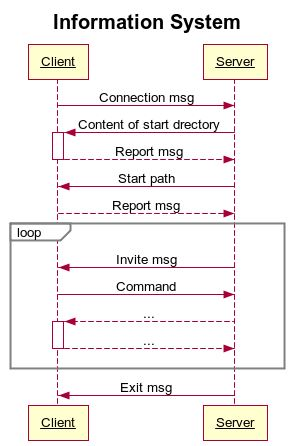
\includegraphics[width=0.5\linewidth]{1.JPG}}
\caption{Основная sequence-диаграмма}
\label{fig:1}
\end{figure}
\begin{figure}[H]
\begin{minipage}[h]{0.49\linewidth}
\center{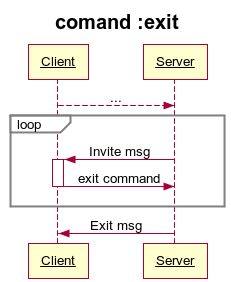
\includegraphics[width=0.5\linewidth]{2.JPG}}
\caption{Итерация с вызовом команды \textit{:exit}}
\label{fig:2}
\end{minipage}
\hfill
\begin{minipage}[h]{0.49\linewidth}
\center{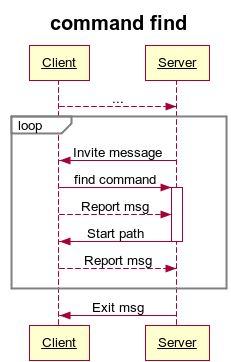
\includegraphics[width=0.5\linewidth]{3.JPG}}
\caption{Итерация с удачным вызовом команды \textit{find}}
\label{fig:3}
\end{minipage}
\end{figure}
\begin{figure}[H]
\center{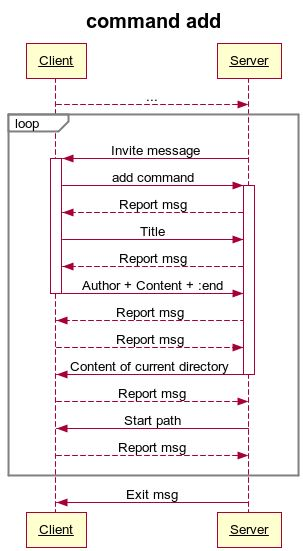
\includegraphics[width=0.5\linewidth]{4.JPG}}
\caption{Итерация с удачным вызовом команды \textit{add}}
\label{fig:4}
\end{figure}
\begin{figure}[H]
\center{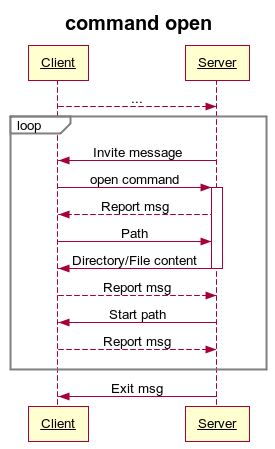
\includegraphics[width=0.5\linewidth]{5.JPG}}
\caption{Итерация с удачным вызовом команды \textit{open}}
\label{fig:5}
\end{figure}

 \FloatBarrier
\section{Тестирование}
\subsection{Описание тестового стенда}
Работа протокола тестируется в двух ОС:
1) Linux debian 3.2.0-4-686-pae \#1 SMP Debian 3.2.63-2+deb7u2 i686 GNU/Linux\\
2) Windows 8.1
\subsection{Тестовый план и результаты тестирования}
План тестирования:

\begin{tabular}{|c|c|}
\hline 
Linux & Linux \\ 
\hline 
Windows & Windows \\ 
\hline 
Windows(Server) & Linux(Client) \\ 
\hline 
Windows(Client) & Linux(Server) \\ 
\hline 
\end{tabular} 


\begin{enumerate}
\item Все возможные команды с разными параметрами()
\begin{itemize}
\item Удачные вызовы
\begin{itemize}
\item :start
\item open (директория(текущая, дочерняя, родительская), файл)
\item  add
\item  :end
\item  find
\item  :exit
\end{itemize}
\item Неудачные вызовы
\begin{itemize}
\item Те же команды с неверными парамерами
\item Несуществующие команды
\end{itemize}
\end{itemize}
\item Ошибки переполнения при вводе команд и их параметров
\item Возможность параллельного соединения клиентов и их конкуренция при сохранении новой статьи
\end{enumerate}

Сервер запускается на Windows системе. К нему по TCP-соединению параллельно подключаются 3 клиента, 1 из которых расположен на Windows ОС.

Во время активной работы клиентов с сервером, последний фиксирует все приходящие и уходящие сообщения и их размер. 
\begin{lstlisting}[language=sh]
...
SEND  [56 bytes]: current path '/home/ks/workspace/InformationSystem/Information System/'
RECV  [4 bytes]: report message  '000'
SEND  [4 bytes]: invitation message '>   '
RECV  [4 bytes]: command 'open'
SEND  [3 bytes]: report message '000'
RECV  [58 bytes]: path to file message '/home/ks/workspace/InformationSystem/Information System/..'
SEND  [100 bytes]: directory content '----------------------|Articles|new.txt|Fairy Tales|first.txt|1.txt|Poems|..|----------------------|'
RECV  [4 bytes]: report message  '000'
SEND  [56 bytes]: current path '/home/ks/workspace/InformationSystem/Information System/'
RECV  [4 bytes]: report message  '000'
SEND  [4 bytes]: invitation message '>   '
RECV  [4 bytes]: command 'open'
SEND  [3 bytes]: report message '000'
RECV  [61 bytes]: path to file message '/home/ks/workspace/InformationSystem/Information System/Poems'
SEND  [71 bytes]: directory content '----------------------|Life|Time|Love|Nature|..|----------------------|'
RECV  [4 bytes]: report message  '000'
SEND  [62 bytes]: current path '/home/ks/workspace/InformationSystem/Information System/Poems/'
RECV  [4 bytes]: report message  '000'
SEND  [4 bytes]: invitation message '>   '
RECV  [4 bytes]: command 'open'
SEND  [3 bytes]: report message '000'
....
\end{lstlisting}

Подключение первого клиента:\\
\begin{enumerate}
\item Два раза подряд ошибочный ввод команды :start
\item На трейтий команда вызвана удачно, как результат, сервер посылает сдержимое корневой директории нформациооной системы
\item Появляется приглашение на ввод команды
\end{enumerate}
\begin{lstlisting}[language=sh]
ks@debian:~/workspace/InformationSystem_ClientTCP/Debug$ ./InformationSystem_ClientTCP 
:sdw
:feueueueueueuue
:start
----------------------
Articles
new.txt
Fairy Tales
first.txt
1.txt
Poems
..
----------------------
>   
\end{lstlisting}
\begin{enumerate}
\item Клиент вызывает команду \textit{open}, чтобы открыть и прочесть файл
\item Сервер пересылает содержимое файла клиенту
\item Клиент пытается зайти в родительскую директорию "корневого" каталога. Доступ запрещен. 
\item Приглашение на ввод команды
\end{enumerate}
\begin{lstlisting}[language=sh]
>   open 1.txt
1
me

Once on December...
>   open ..
----------------------
Articles
new.txt
Fairy Tales
first.txt
1.txt
Poems
..
----------------------
>  
\end{lstlisting}

\begin{enumerate}
\item Клиент переходит в раздел Poems/Love
\item Клиент вводит команду поиска статей по имени автора \textit{find}. Вводит часть имени: \textit{shak}
\item Клиент отправляет команду \textit{open}, чтобы открыть найденный файл, и получает его содержимое
\item Клиент запрашивает содержимое текущего раздела
\end{enumerate}

\begin{lstlisting}[language=sh]
>   open Poems
----------------------
Life
Time
Love
Nature
..
----------------------
>   open Love
----------------------
Love is my Sin.txt
Love.txt
..
----------------------
>   find shak
Search results for author: shak
----------------------
William Shakespeare
:    Love is my Sin.txt
----------------------
>   open Love is my Sin.txt
Love is my Sin
William Shakespeare

CXLII.

Love is my sin and thy dear virtue hate,
Hate of my sin, grounded on sinful loving:
O, but with mine compare thou thine own state,
And thou shalt find it merits not reproving;
Or, if it do, not from those lips of thine,
That have profaned their scarlet ornaments
And seal'd false bonds of love as oft as mine,
Robb'd others' beds' revenues of their rents.
Be it lawful I love thee, as thou lovest those
Whom thine eyes woo as mine importune thee:
Root pity in thy heart, that when it grows
Thy pity may deserve to pitied be.
If thou dost seek to have what thou dost hide,
By self-example mayst thou be denied!
>   open .
----------------------
Love is my Sin.txt
Love.txt
..
\end{lstlisting}


\begin{enumerate}
\item Клиент1 вводит команду \textit{add} чтобы создать статью с заголовкам "3"
\item В это время подключается Клиент2 и пытается создать статью с таким же заголовком 
\item Клиент2 закончил ввод содержимого быстрее, в результате Клиент1 после ввода своего содержимого получает ошибку, его введенные данные теряются
\item Клиент1 обижается и уходит, послав команду \textit{:exit}
\end{enumerate}

\begin{lstlisting}[language=sh]
>   add
3
Input author: me
name's read: 3 [1 bytes]
author's read: me [1 bytes]
Put content:
[0 of 3840]  I'm fine! And you?
:end
!Such file already exist

----------------------
3.txt
Articles
new.txt
Fairy Tales
first.txt
1.txt
Poems
..
----------------------
>   open 3.txt
3
he

Hello!
How are you!

>   :exit
Bye-bye!!!
\end{lstlisting}

\begin{lstlisting}[language=sh]
>   add 3
Input author: he
name's read: 3 [1 bytes]
author's read: he [1 bytes]
Put content:
[0 of 3840]  Hello!
How are you!
:end

----------------------
3.txt
Articles
new.txt
Fairy Tales
first.txt
1.txt
Poems
..
----------------------
>   open 3.txt
3
he

Hello!
How are you!
\end{lstlisting}

\chapter{Реализация для работы по протоколу UDP}
\section{Прикладной протокол и ахитектура}
Реализация UDP протокола отличается от TCP только использованием функций recv/recvfrom и send/sendto. А также тем, что в данном случае не удалось реализовать многопоточность. Были попытки установления параллельного подключения клиентов с использованием мьютексов. Однако эи попытки не увенчались успехом. В данной реализации используется последовательное подключение клиентов: Каждый новый ждет завершения работы предыдущего клиента.

\section{Тестирование}
\subsection{Описание тестового стенда}
Работа протокола тестируется в двух ОС:
1) Linux debian 3.2.0-4-686-pae \#1 SMP Debian 3.2.63-2+deb7u2 i686 GNU/Linux\\
2) Windows 8.1
\subsection{Тестовый план и результаты тестирования}

\begin{enumerate}
\item Ввод несуществующих команд
\item удачный и неудачный поиск
\item Тест на переполнение при вводе новой статьи
\end{enumerate}
Сервер запускается на UNIX ОС. К нему по UDP-соединению последовательно подключаются 2 клиента: один из ОС Windows, другой - из Unix.

\begin{enumerate}
\item Клиент1 подсоединяется к порту 5001 и серверу с ip-адресом 172.16.51.83 командой  \textit{:start}
\item Неудачный поиск командой \textit{find}
\item Удачный поиск по имени автора
\end{enumerate}


\begin{lstlisting}[language=sh]
C:\Users\Kseniya\workspace\client_udp\Debug>client_udp.exe -p:5001 -i:172.16.51.83
:start
----------------------
Literature
second.txt
first.txt
1.txt
..
----------------------
>   open 1.txt
title:  STORY
author: PUSHKIN
Hello, everybody!
LALAL
>   find pusjkin
There are no articles of pusjkin
>   find pushkin
Search results for author: pushkin
----------------------
author: PUSHKIN
:    1.txt
----------------------
>
\end{lstlisting}

\begin{enumerate}
\item Клиент1 переходит в раздел Literature
\item Вводит команду \textit{add}, чтобы добавить статью в систему 
\item Вызов переполнения при вставке большого куска текста
\item Проверка  возможности чтения добавленной статьи
\item Попытка открыть несуществующий файл/раздел
\end{enumerate}
\begin{lstlisting}[language=sh]
>   open Literature
----------------------
story.txt
Rapunzel.txt
..
Clever Hans.txt
----------------------
>   add Something
Input author: Hans Chrustian Andersen
name's read: Something [9 bytes]
author's read: Hans Chrustian Andersen [9 bytes]
Put content:
[0 of 3840]  MEAN to be somebody, and do something useful in the world," said the eldest of five bro
thers. "I don't care how humble my position is, so that I can only do some good, which will be somet
hing. I intend to be a brickmaker; bricks are always wanted, and I shall be really doing something."
"Your 'something' is not enough for me," said the second brother; "what you talk of doing is nothing
 at all, it is journeyman's work, or might even be done by a machine. No! I should prefer to be a bu
ilder at once, there is something real in that. A man gains a position, he becomes a citizen, has hi
s own sign, his own house of call for his workmen: so I shall be a builder. If all goes well, in tim
e I shall become a master, and have my own journeymen, and my wife will be treated as a master's wif
.....
ich formed a dyke on the sea-coast, a poor woman named Margaret wished to build herself a house, so
all the imperfect bricks were given to her, and a few whole ones with them; for the eldest brother w
as a kind-hearted man, although he never achieved anything higher than making bricks. The poor woman
 built herself a little house-it was small and narrow, and the window was quite crooked, the door to
o low, and the straw roof might have been better thatched. But still it was a shelter, and from with
[3840 of 3840]  !Type less or :end
[3840 of 3840]  !Type less or :end
[3840 of 3840]  !Type less or :end
[3840 of 3840]  !Type less or :end
[3840 of 3840]  !Type less or :end
[3840 of 3840]  !Type less or :end
[3840 of 3840]  !Type less or :end
[3840 of 3840]  :end

----------------------
story.txt
Rapunzel.txt
Something.txt
..
Clever Hans.txt
----------------------
>   open Something.txt
Something
Hans Chrustian Andersen

MEAN to be somebody, and do something useful in the world," said the eldest of five brothers. "I don
't care how humble my position is, so that I can only do some good, which will be something. I inten
d to be a brickmaker; bricks are always wanted, and I shall be really doing something."

"Your 'something' is not enough for me," said the second brother; "what you talk of doing is nothing
 at all, it is journeyman's work, or might even be done by a machine. No! I should prefer to be a bu
ilder at once, there is something real in that. A man gains a position, he becomes a citizen, has hi
s own sign, his own house of call for his workmen: so I shall be a builder. If all goes well, in tim
e I shall become a master, and have my own journeymen, and my wife will be treated as a master's wif
e. This is what I call something."

"I call it all nothing," said the third; "not in reality any position. There are many in a town far
above a master builder in position. You may be an upright man, but even as a master you will only be
...
 always be men like these five brothers. And what became of them? Were they each nothing or somethin
g? You shall hear; it is quite a history.

The eldest brother, he who fabricated bricks, soon discovered that each brick, when finished, brough
t him in a small coin, if only a copper one; an
>   open ,'
!No such file or directory
\end{lstlisting}
\chapter{Выводы}
В результате выполнения данных заданий можно сделать вывод, что для предложенного протокола гораздо удобнее испоьзовать TCP-соединение. Это сязано с тем, что TCP является надеждным соединение, в отличие от UDP, а так как работа информационной системы связана с передачей больших текстовых сообщений, то выбор TCP будет наиболее предпочтителен. Еще одним приемуществом использования TCP является возможность реализации многопоточности, чего не удалось достичь при использовании UDP.

\chapter*{Приложения}
\section*{Описание среды разработки}
Версии ОС, компиляторов, утилит, и проч., которые использовались в процессе разработки
\section*{Листинги}
\subsection*{UNIX}
\subsection*{TCP Server}
main.c
\lstinputlisting[]
{/home/user/workspace/listings/unix/tcp_server/main.c}
article.h
\lstinputlisting[]
{/home/user/workspace/listings/unix/tcp_server/article.h}
article.c
\lstinputlisting[]
{/home/user/workspace/listings/unix/tcp_server/article.c}
\subsection*{TCP Client}
main.c
\lstinputlisting[]
{/home/user/workspace/listings/unix/tcp_client/main.c}
\subsection*{UDP Server}
main.c
\lstinputlisting[]
{/home/user/workspace/listings/unix/udp_server/main.c}
article.h
\lstinputlisting[]
{/home/user/workspace/listings/unix/udp_server/article.h}
article.c
\lstinputlisting[]
{/home/user/workspace/listings/unix/udp_server/article.c}
\subsection*{UDP Client}
main.c
\lstinputlisting[]
{/home/user/workspace/listings/unix/udp_client/main.c}
\subsection*{WINDOWS}
\subsection*{TCP Server}
main.c
\lstinputlisting[]
{/home/user/workspace/listings/win/tcp_server/main.c}
article.h
\lstinputlisting[]
{/home/user/workspace/listings/win/tcp_server/article.h}
article.c
\lstinputlisting[]
{/home/user/workspace/listings/win/tcp_server/article.c}
\subsection*{TCP Client}
main.c
\lstinputlisting[]
{/home/user/workspace/listings/win/tcp_client/main.c}
\subsection*{UDP Server}
main.c
\lstinputlisting[]
{/home/user/workspace/listings/win/udp_server/main.c}
article.h
\lstinputlisting[]
{/home/user/workspace/listings/win/udp_server/article.h}
article.c
\lstinputlisting[]
{/home/user/workspace/listings/win/udp_server/article.c}
\subsection*{UDP Client}
main.c
\lstinputlisting[]
{/home/user/workspace/listings/win/udp_client/main.c}
%\subsection*{Файл сборки Makefile}
%\lstinputlisting[language=make,label={Makefile}]
%{/home/user/workspace/tcp_server/Makefile}
%\todo[inline]{Не забыть вставить все исходники}
\end{document}